\subsection{\label{sec:data.lepton}General Features of Lepton Data in \desg{g12}}

To identify electrons and positrons properly in \abbr{CLAS}, quantities obtained from the \abbr{CC} and \abbr{EC} are used to reject charged pions. The \abbr{CC} collects the number of photo-electrons caused by Cerenkov radiation and the \abbr{EC} records the energy deposition of electrons/positrons as well as photons. A previous \abbr{CLAS} experiment \desg{g7} analyzed the properties of medium modifications from the decay of vector mesons through the lepton decay channel. This experiment derived a set of cits for identifying electron/positrons pairs in \abbr{CLAS} by employing specific cuts to the number of photo-electrons (\abbr{NPE}) detected in the \abbr{CC}, a match in azimuthal angle $\phi$ from a charged track in the \abbr{DC} to the $\phi$ of the \abbr{CC}, as well as comparing the momentum of the charged track to the energy deposited in the \abbr{EC}. These cuts can be found in Table~\ref{tab:ISLEP_cuts}.
\begin{table}[h!]
\begin{minipage}{\textwidth}
\begin{center}
\begin{singlespacing}

\caption[Electron/Positron PID Cuts]{\label{tab:ISLEP_cuts}Cuts applied to the \emph{CC} and \emph{EC} to perform electron/positron \emph{PID}. Table source:~\cite{clas.thesis.kunkel} \vspace{0.75mm}}

\begin{tabular}{c|c|c}

\hline
Subsystem & Quantity & Cut \\
\hline
\multirow{2}{*}{\emph{CC}}  & \# of photo-electrons (\emph{NPE})  & \emph{NPE} $>$ 2.5 \\
 &  \emph{DC} $\phi$ \& \emph{CC} $\phi$  & \emph{DC} $\phi$ = \emph{CC} $\phi$ \\
\hline
\multirow{2}{*}{\emph{EC}}  & q$^{\pm}$ momentum threshold (p$\mathrm{_{thres}}$) & \multirow{2}{*}{p$\mathrm{_{thres}^{high}} < \ $E$\mathrm{_{calo}} <$ p$\mathrm{_{thres}^{low}}$ } \\
&  \& \emph{EC} deposited energy (E$\mathrm{_{calo}}$) & \\
\hline \hline
\end{tabular}
\end{singlespacing}
\end{center}
\end{minipage}
\end{table}

To validate the \desg{g7} electron/positron \abbr{PID} scheme for \desg{g12}, a comparison of  the \abbr{CC} and \abbr{EC} quantities was performed for all charged tracks \abbr{CC}/\abbr{EC} hit signatures and while selecting events from π$^0$ decay. To separate the π$^0$ events from the π$^+$π$^-$ events, all charged pions were assigned the mass of electrons and cuts were placed on the missing energy of \mbox{γ p$\rightarrow$p e$^+$ e$^-$} as well as a cut on the missing mass squared of \mbox{γ p$\rightarrow$ p}, values found in Table~\ref{tab:lep_cuts}. A graphical depiction of the cuts applied to separate π$^0$ events from the π$^+$π$^-$ events is seen in Fig.~\ref{fig:islep.cuts}.
\begin{table}[htpb]
\begin{minipage}{\textwidth}
\begin{center}
\begin{singlespacing}

\caption[Cuts To Separate $\pi^0$ from $\pi^{+}\pi^{-}$ for \emph{PID} Validation]{\label{tab:lep_cuts}Cuts applied to separate $\pi^0$ events from $\pi^{+}\pi^{-}$ events. Table source:~\cite{clas.thesis.kunkel} \vspace{0.75mm}}

\begin{tabular}{c|c|c}

\hline
Cut Topology & Topology Quantity & Value  \\
\hline
$\gamma p \rightarrow p e^+ e^-$ & Missing Energy ($\mathrm{M_E}$) & $>0.075$~GeV \\
\hline
\multirow{2}{*}{$\gamma p \rightarrow p $}  & \multirow{2}{*}{Missing mass squared ($\mathrm{M_x^2}$)} & $<$ 0.0779~GeV$^2$ for $\pi^0$ events \\
&  & $>$ 0.0779~GeV$^2$ for $\pi^{+}\pi^{-}$ events\\
\hline \hline
\end{tabular}

\end{singlespacing}
\end{center}
\end{minipage}
\end{table}

The values of the threshold momentum are calculated from empirical studies and are based upon calculations using the momentum obtained from the \abbr{DC}$p$ under the following criteria;
\begin{align}
\mathrm{p_{thres}^{low}} = \alpha p *(p+EC_{P\_LO})/p \nonumber \\
\mathrm{p_{thres}^{high}} = \alpha p *(p+EC_{P\_HIGH})/p \nonumber
\end{align}
where $EC_{P\_LO} = -0.3$, $EC_{P\_HIGH} = 0.5$ and
\begin{align}
\alpha p =
\begin{cases}
.23*p + .071p^2 - .032p^3, & p<1.0 \text{~GeV} \\
0.272p, & p>1.0 \text{~GeV} \\
\end{cases}\nonumber
\end{align}


\begin{figure}\begin{center}
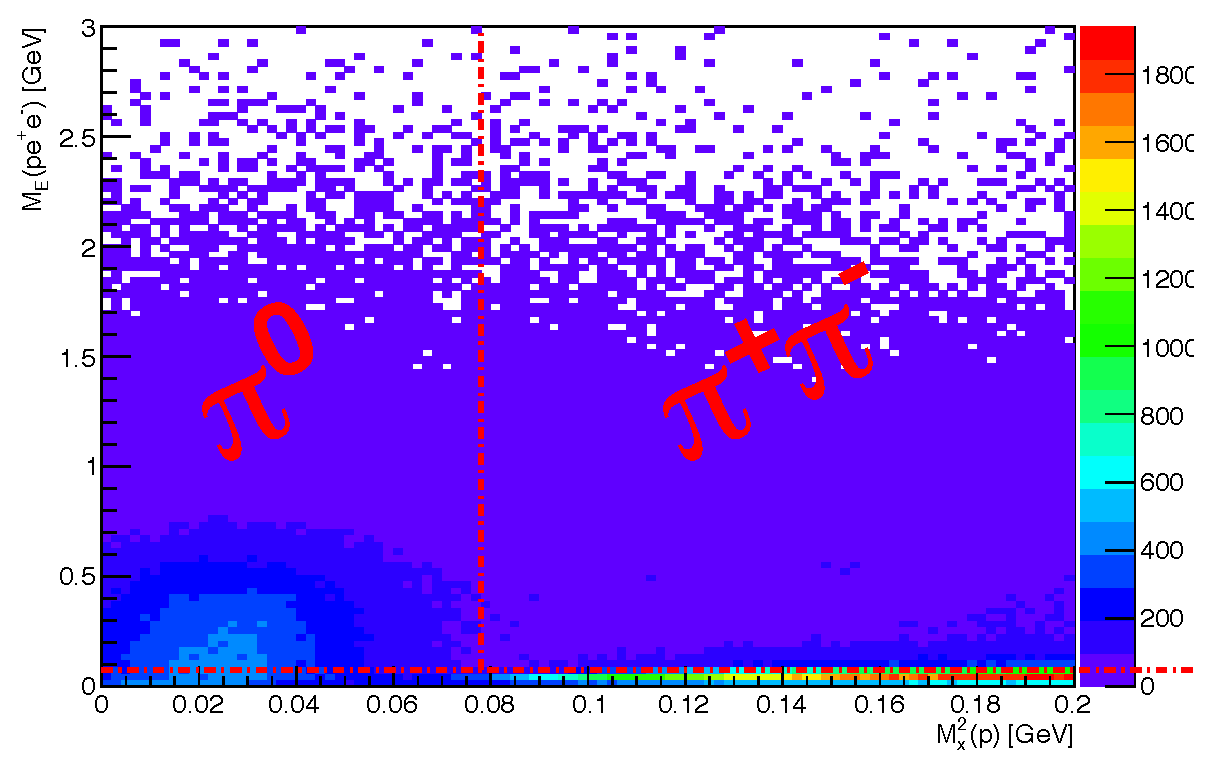
\includegraphics[width=0.4\textwidth]{figures/lepton/Lepfeature_cuts.eps}
\caption[Cuts Applied to Isolate π$^0$ and π$^+$ π$^-$ for \abbr{PID} Validation]{\label{fig:islep.cuts}Plot of missing mass squared of off proton (horizontal) vs. missing energy of proton e$^+$e$^-$ (vertical). The red dashed vertical line depicts the π$^+$π$^-$ threshold mass cut while the horizontal red dashed line represents the missing energy cut-off used to sepertate π$^+$π$^-$ from π$^0$.  Image source:~\cite{clas.thesis.kunkel}}
\end{center}\end{figure}


There are more and more restrictive cuts one can always do to try to clean up a lepton signal, but the general \abbr{CC}, \abbr{TOF}, and \abbr{EC}$_\mathrm{total}$ are the most robust. After that you can make further cuts on \abbr{EC}$_\mathrm{inner}$ and/or \abbr{EC}$_\mathrm{outer}$ at the users discretion. The g7 lepton cuts were the standard isLepton(), plus a $>45$~MeC \abbr{EC}$_\mathrm{inner}$ cut, see Ref.~\cite{clas.nasseripour}.


\subsubsection{\label{sec:data.lepton.cc}\abbr{CC} Comparison}

The \abbr{NPE} measured by the \abbr{CC} for all positron/electron (e$^+$/e$^-$) candidates can be seen in Fig~\ref{fig:islep.CC}. The sharp decline prior to 2.5 \abbr{NPE} is due to photo-electrons created by electron/positrons, pions traveling through the \abbr{CC} or pions producing delta-electrons which pass through the \abbr{CC}. Delta-electrons are created as an effect of the ionization of gases that could be present when the pion travels through the \abbr{DC}. These types of electrons are typically lower in momentum than the electrons obtained from particle decays in \abbr{CLAS} and thus should emit less \abbr{NPE} per unit length.

Through mass conservation the particles for the π$^0$ events must be e$^+$/e$^-$ pairs. In comparison to fig.~\ref{fig:islep.CC}, fig.~\ref{fig:islep.CC1} plots the \abbr{NPE} measured by the \abbr{CC} for all e$^+$/e$^-$ pairs for π$^0$ events selected as shown in fig.~\ref{fig:islep.cuts}. It can be seen that the sharp decline prior to \abbr{NPE} = 2.5 is reduced leaving mostly electrons or positrons signatures in the \abbr{CC} concluding that the \desg{g7} \abbr{CC} \abbr{NPE} cut is valid for identifying e$^+$/e$^-$ pairs while rejecting π$^+$/π$^-$ pairs.

Using the current cuts of \abbr{NPE} and hit angle, the suppression of di-leptons was sufficient without including additional cuts on the \abbr{CC} such as a timing comparison to the \abbr{TOF}. This method of lepton \abbr{PID}, involving di-leptons, was established during the \textit{g7} run period. Further \textit{g12} analyses that involve single lepton \abbr{PID} could include this as a cut.

%
\begin{figure}\begin{center}
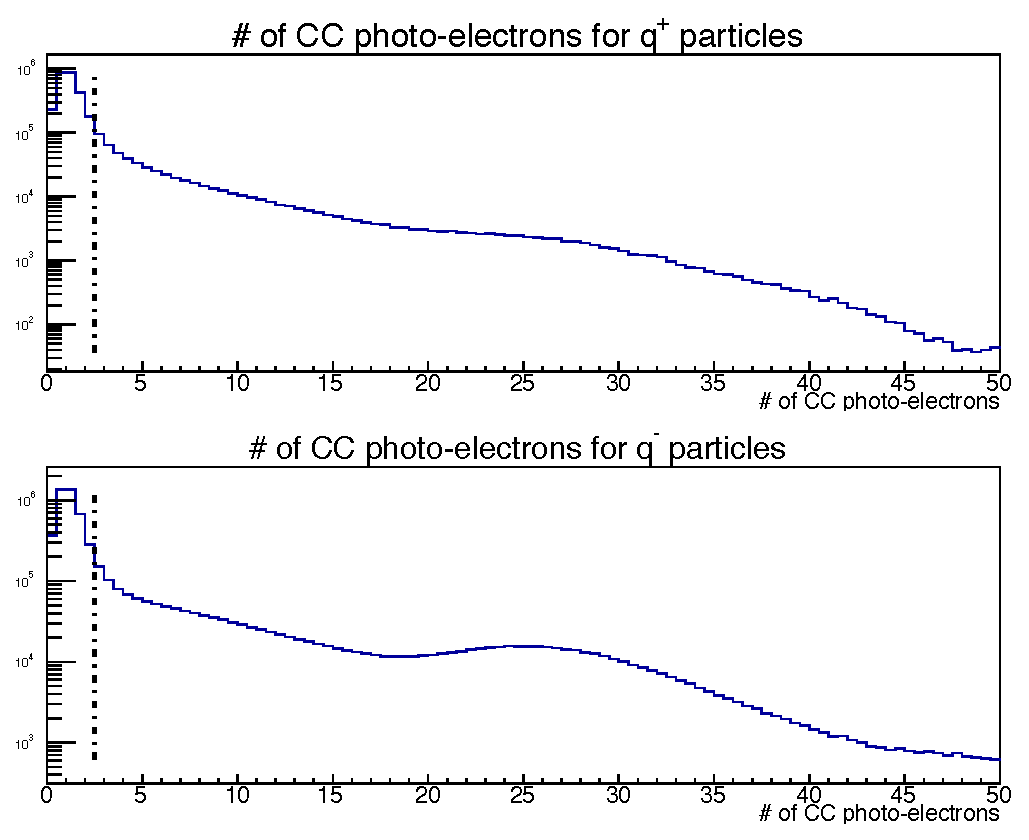
\includegraphics[width=0.4\textwidth]{figures/lepton/CC_nPE.eps}
\caption[Number of Photo-electrons Measured by \abbr{CC} for All e$^-$ and e$^+$ Candidates]{\label{fig:islep.CC}Plot of \abbr{NPE} measured by \abbr{CLAS} \abbr{CC} subsystem for positron/electron candidates top/bottom respectively. The dashed dotted vertical line depicts the cut applied if using the \desg{g7} lepton \abbr{PID} scheme. Image source:~\cite{clas.thesis.kunkel}}
\end{center}\end{figure}

\begin{figure}\begin{center}
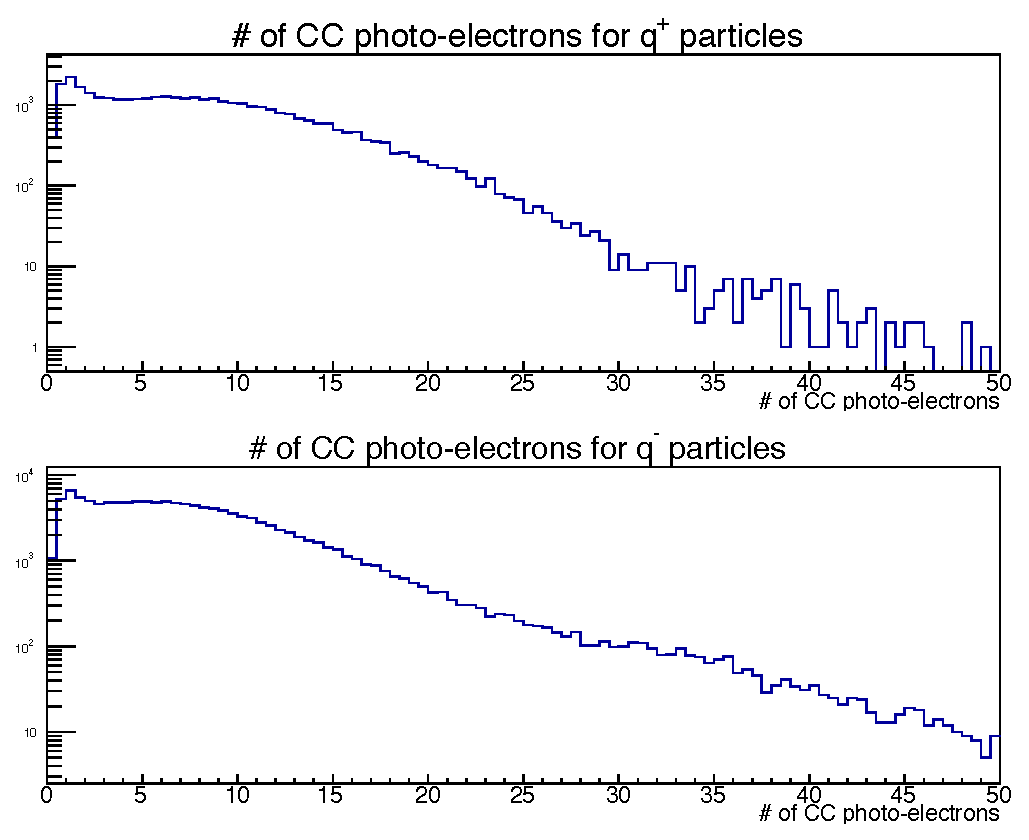
\includegraphics[width=0.4\textwidth]{figures/lepton/CC_NPEcut.eps}
\caption[Number of Photo-electrons Measured by \abbr{CC} for π$^0$ Events]{\label{fig:islep.CC1}Plot of \abbr{NPE} measured by \abbr{CLAS} \abbr{CC} subsystem when selecting π$^0$ events seen in Fig~\ref{fig:islep.cuts}, positron/electron candidates top/bottom respectively. Image source:~\cite{clas.thesis.kunkel}}
\end{center}\end{figure}

\FloatBarrier






\subsubsection{\label{sec:data.lepton.ec}\abbr{EC} Comparison}

Similarly to the \abbr{CC} comparison, figures~\ref{fig:islep.pimEClow},~\ref{fig:islep.pimEChigh},~\ref{fig:islep.pipEClow},~\ref{fig:islep.pipEChigh} depict the  p$\mathrm{_{thres}^{low}}$ and  p$\mathrm{_{thres}^{low}}$ cuts listed in  Table~\ref{tab:ISLEP_cuts} for the q$^-$ and q$^+$ tracks respectively. After π$^0$ event selection, seen in figures~\ref{fig:islep.pimEC},~\ref{fig:islep.pimECcut} ,~\ref{fig:islep.pipEC} ,~\ref{fig:islep.pipECcut}, the bulk of e$^+$/e$^-$ events reside within the region of the cut acceptance therefore it is evident that the \desg{g7} \abbr{EC} cuts are valid for identifying e$^+$/e$^-$ pairs. The following four plots are for electron($e^-$) \abbr{PID} validation of the \desg{g7} \abbr{EC} cuts described in Table~\ref{tab:ISLEP_cuts}.
%
\begin{figure}\begin{center}
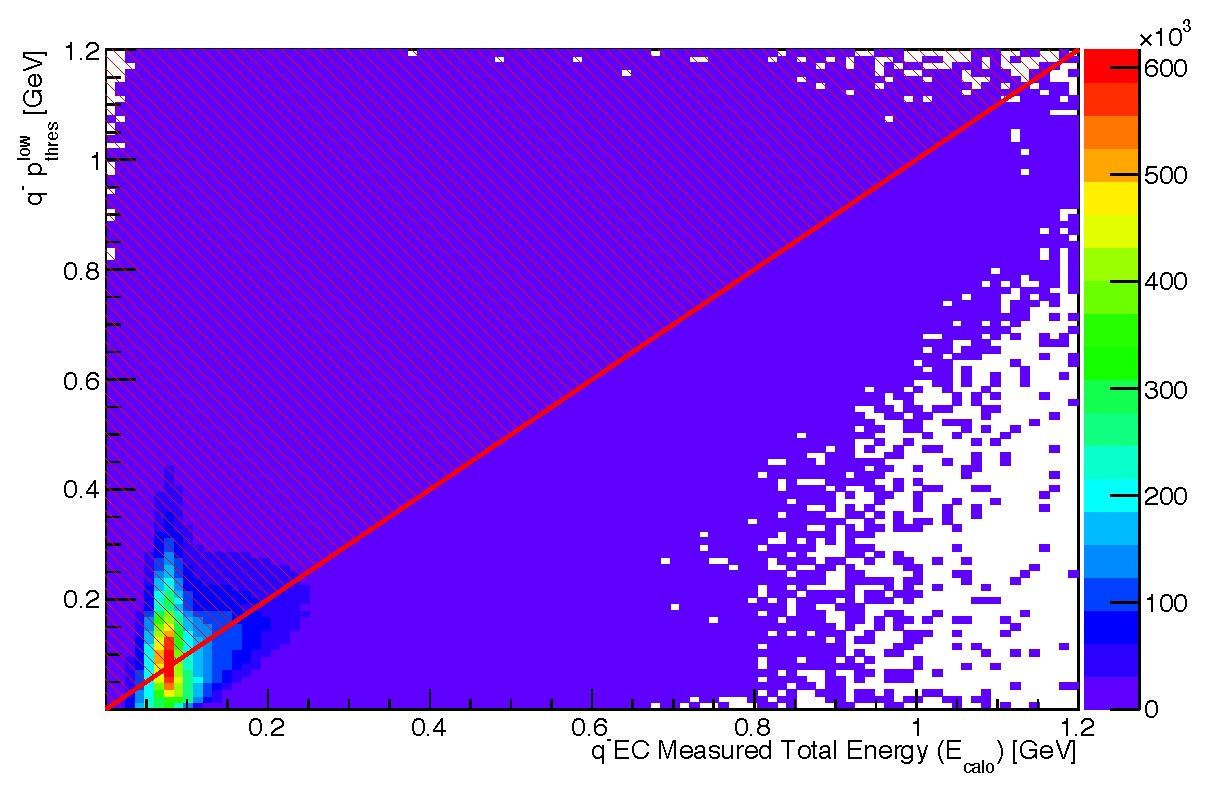
\includegraphics[width=0.4\textwidth]{figures/lepton/Pim_EClow.eps}
\caption[\abbr{EC} Deposited Energy Comparison to Lower Threshold Track Momentum for q$^-$ Tracks]{\label{fig:islep.pimEClow}Plot of energy deposited measured by \abbr{EC} vs. track momentum p$\mathrm{_{thres}^{low}}$ for negative charged tracks. The red region depicts the cut that would reject events in the \desg{g7} lepton \abbr{EC} \abbr{PID} scheme. Image source:~\cite{clas.thesis.kunkel}}
\end{center}\end{figure}

\begin{figure}\begin{center}
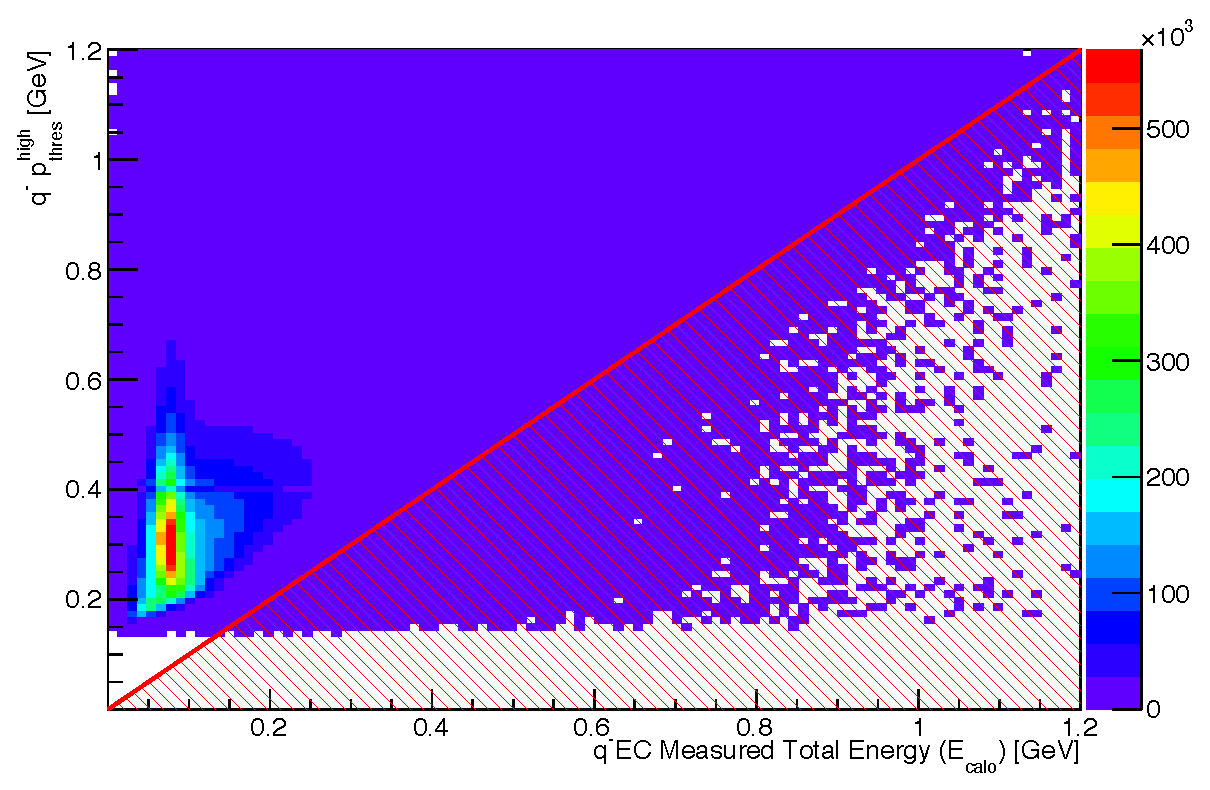
\includegraphics[width=0.4\textwidth]{figures/lepton/Pim_EChigh.eps}
\caption[\abbr{EC} Deposited Energy Comparison to Upper Threshold Track Momentum for q$^-$ Tracks]{\label{fig:islep.pimEChigh}Plot of energy deposited measured by \abbr{EC} vs. track momentum p$\mathrm{_{thres}^{high}}$ for negative charged tracks. The red region depicts the cut that would reject events in the \desg{g7} lepton \abbr{EC} \abbr{PID} scheme. Image source:~\cite{clas.thesis.kunkel}}
\end{center}\end{figure}


\begin{figure}\begin{center}
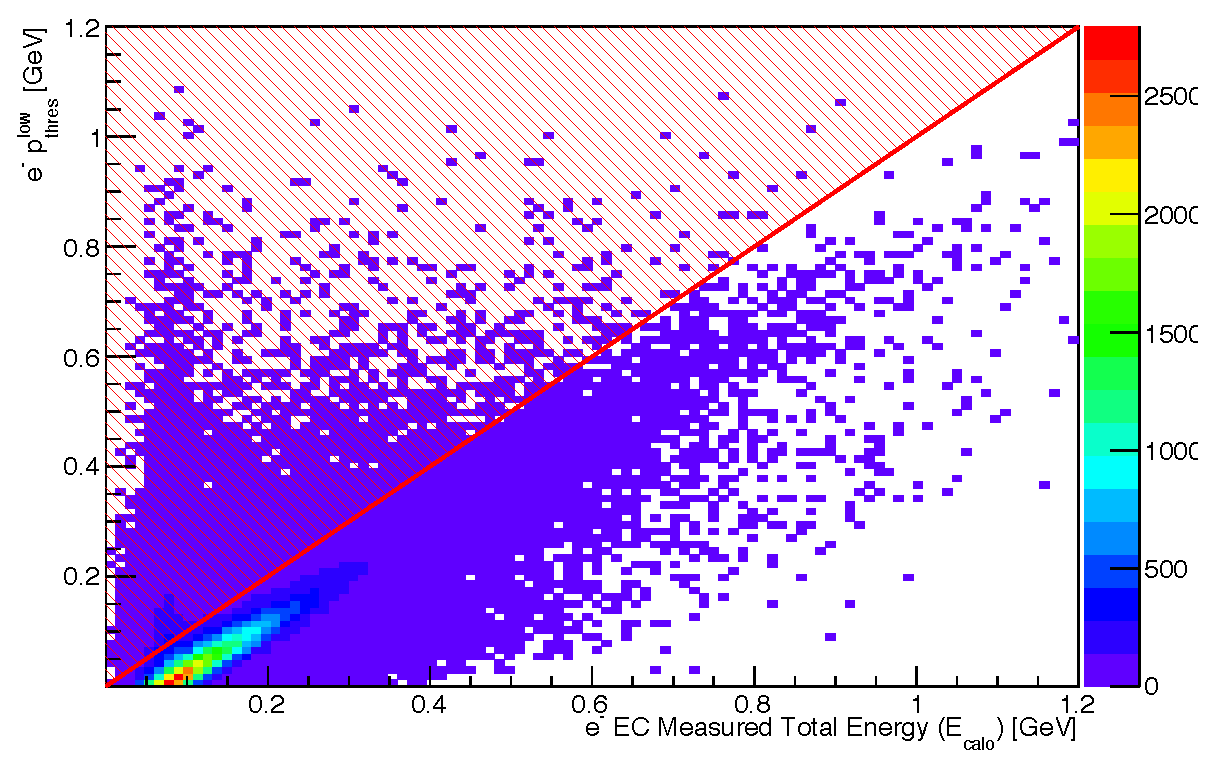
\includegraphics[width=0.4\textwidth]{figures/lepton/Pim_EClowcut.eps}
\caption[\abbr{EC} Deposited Energy Comparison to Track Momentum for e$^-$ Candidates]{\label{fig:islep.pimEC}Plot of energy deposited measured by \abbr{EC} vs. track momentum p$\mathrm{_{thres}^{low}}$ for electrons from π$^0$ events without the \desg{g7} lepton \abbr{EC} \abbr{PID} scheme applied. The red region depicts the cut that would reject events in the \desg{g7} lepton \abbr{EC} \abbr{PID} scheme. Image source:~\cite{clas.thesis.kunkel}}
\end{center}\end{figure}

\begin{figure}\begin{center}
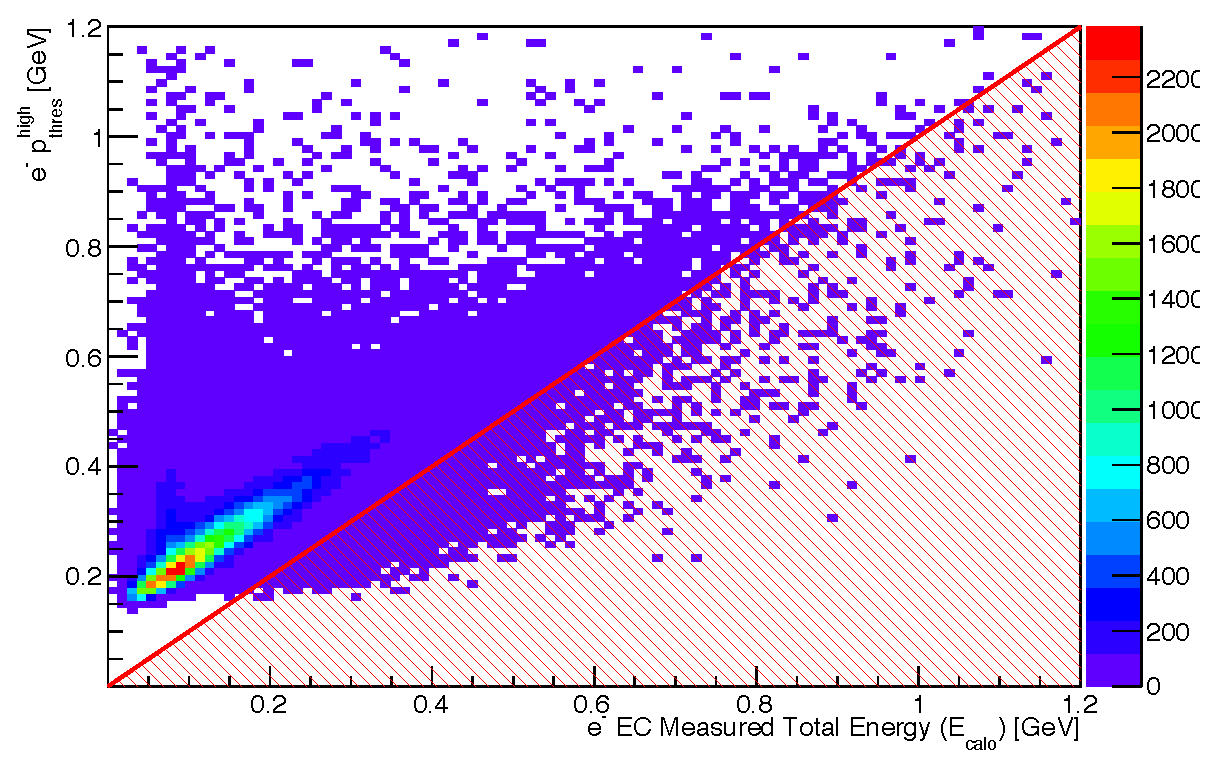
\includegraphics[width=0.4\textwidth]{figures/lepton/Pim_EChighcut.eps}
\caption[\abbr{EC} Deposited Energy Comparison to Track Momentum for e$^-$ from π$^0$ Events]{\label{fig:islep.pimECcut}Plot of energy deposited measured by \abbr{EC} vs. track momentum p$\mathrm{_{thres}^{high}}$ for electrons from π$^0$ events without the \desg{g7} lepton \abbr{EC} \abbr{PID} scheme applied. The red region depicts the cut that would reject events in the \desg{g7} lepton \abbr{EC} \abbr{PID} scheme. Image source:~\cite{clas.thesis.kunkel}}
\end{center}\end{figure}

Figures~\ref{fig:islep.pipEClow}--\ref{fig:islep.pipECcut} are for positron (e$^+$) \abbr{PID} validation of the \desg{g7} \abbr{EC} cuts described in Table~\ref{tab:ISLEP_cuts}.

\begin{figure}\begin{center}
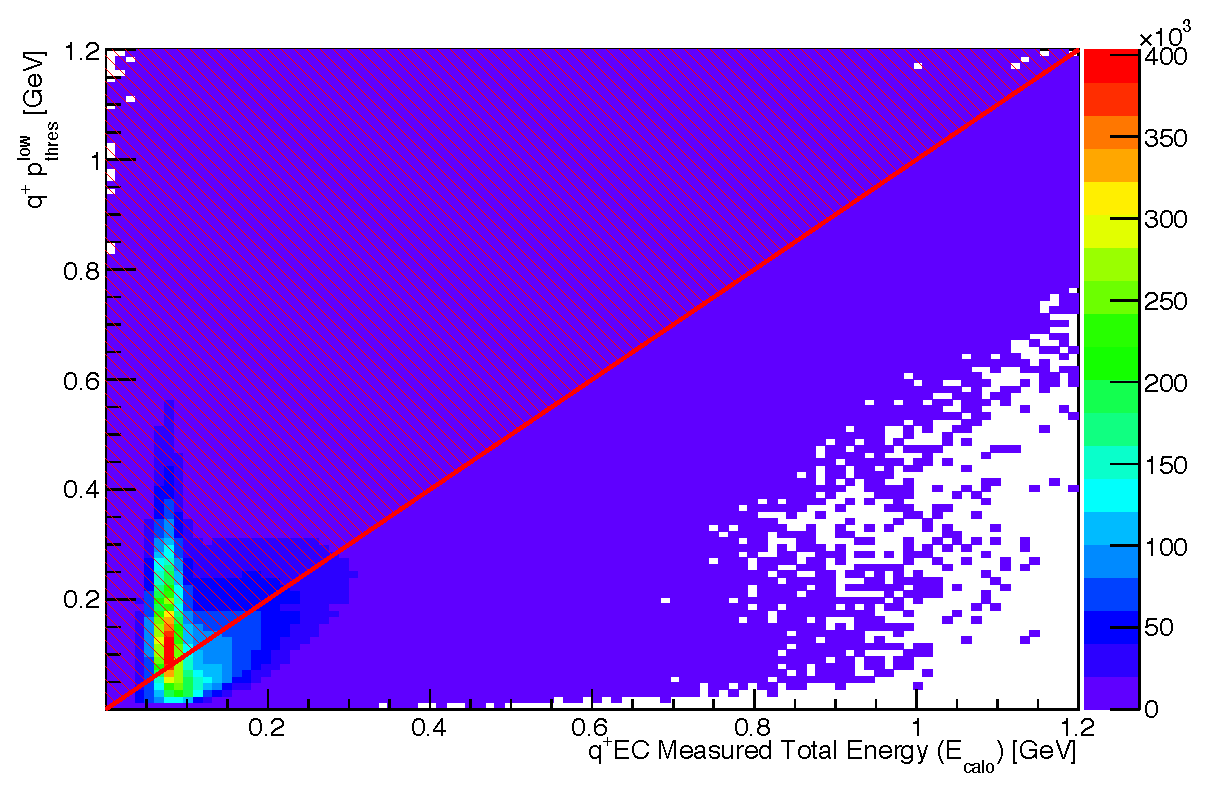
\includegraphics[width=0.45\columnwidth]{figures/lepton/Pip_EClow.eps}
\caption[\abbr{EC} Deposited Energy Comparison to Lower Threshold Track Momentum for q$^+$ Tracks]{\label{fig:islep.pipEClow}Plot of energy deposited measured by \abbr{EC} vs. track momentum p$\mathrm{_{thres}^{low}}$ for positive charged tracks. The red region depicts the cut that would reject events in the \desg{g7} lepton \abbr{EC} \abbr{PID} scheme. Image source:~\cite{clas.thesis.kunkel}}
\end{center}\end{figure}

\begin{figure}\begin{center}
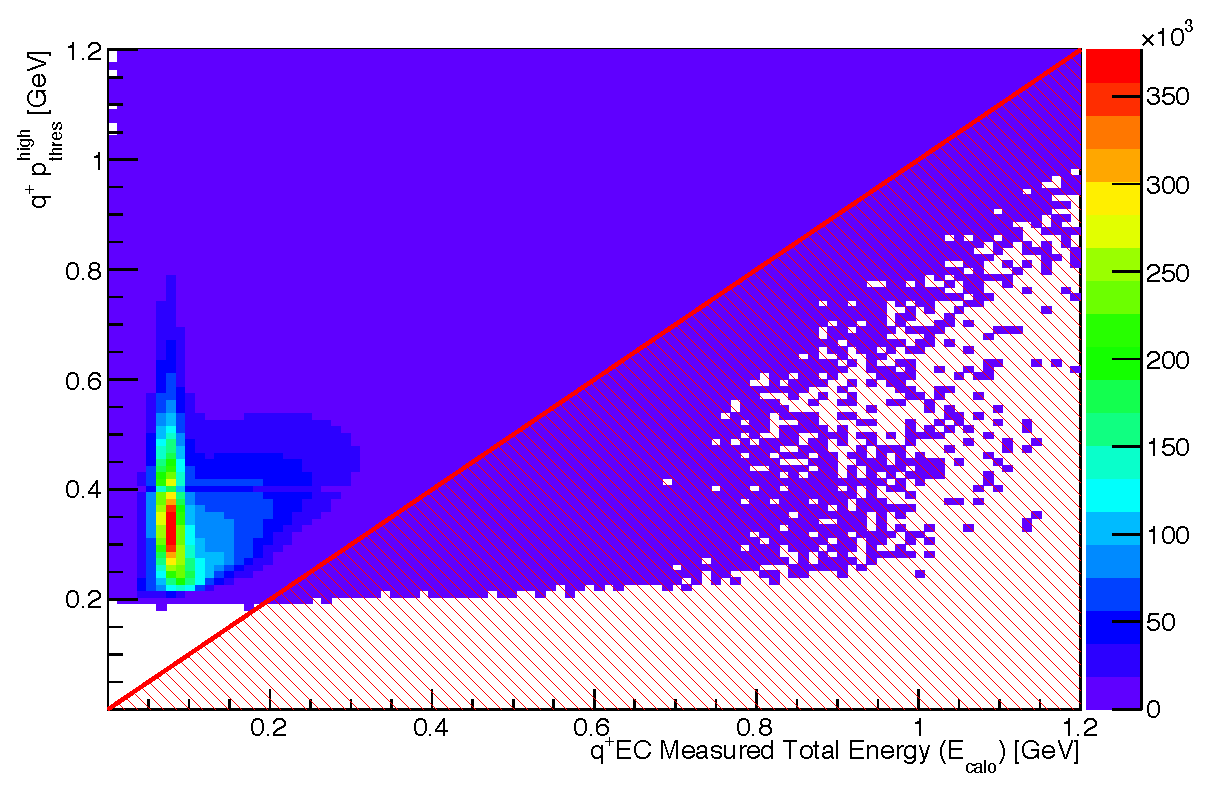
\includegraphics[width=0.45\columnwidth]{figures/lepton/Pip_EChigh.eps}
\caption[\abbr{EC} Deposited Energy Comparison to Upper Threshold Track Momentum for q$^+$ Tracks]{\label{fig:islep.pipEChigh}Plot of energy deposited measured by \abbr{EC} vs. track momentum p$\mathrm{_{thres}^{high}}$ for positive charged tracks. The red region depicts the cut that would reject events in the \desg{g7} lepton \abbr{EC} \abbr{PID} scheme. Image source:~\cite{clas.thesis.kunkel}}
\end{center}\end{figure}

\begin{figure}\begin{center}
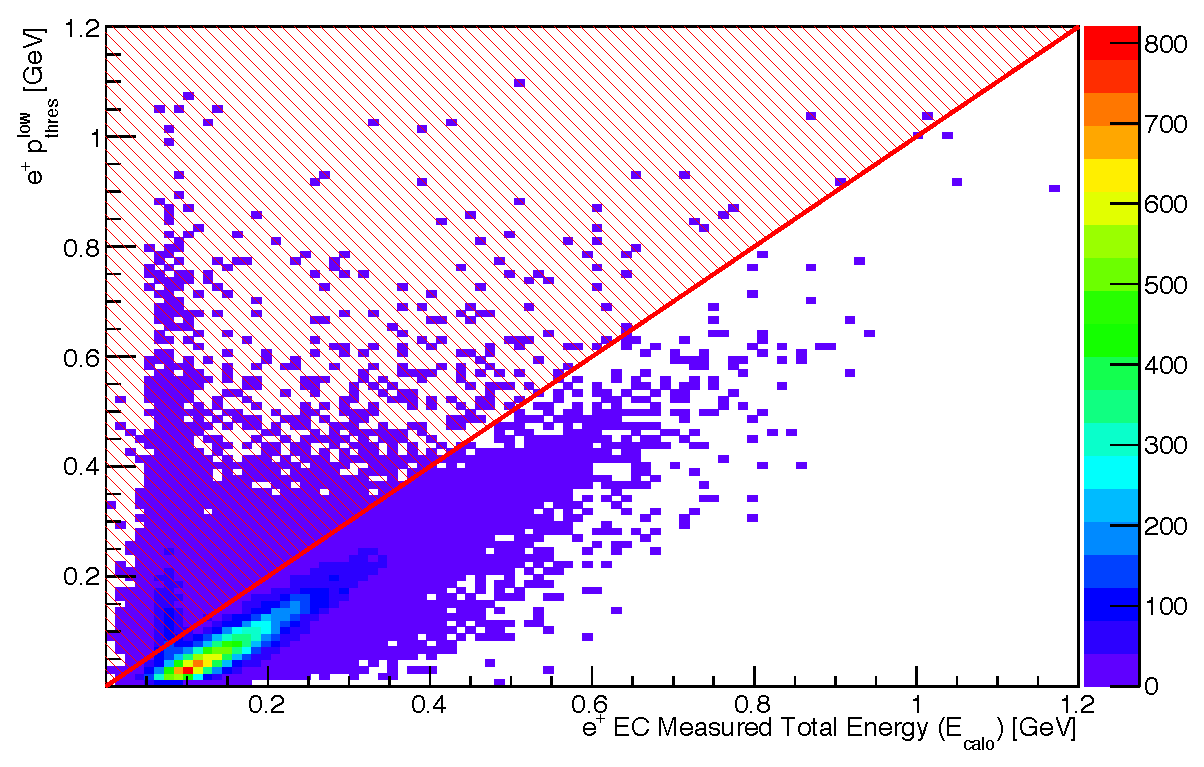
\includegraphics[width=0.45\columnwidth]{figures/lepton/Pip_EClowcut.eps}
\caption[\abbr{EC} Deposited Energy Comparison to Track Momentum for e$^+$ Candidates]{\label{fig:islep.pipEC}Plot of energy deposited measured by \abbr{EC} vs. track momentum p$\mathrm{_{thres}^{low}}$ for positrons from π$^0$ events without the \desg{g7} lepton \abbr{EC} \abbr{PID} scheme applied. The red region depicts the cut that would reject events in the \desg{g7} lepton \abbr{EC} \abbr{PID} scheme. Image source:~\cite{clas.thesis.kunkel}}
\end{center}\end{figure}

\begin{figure}\begin{center}
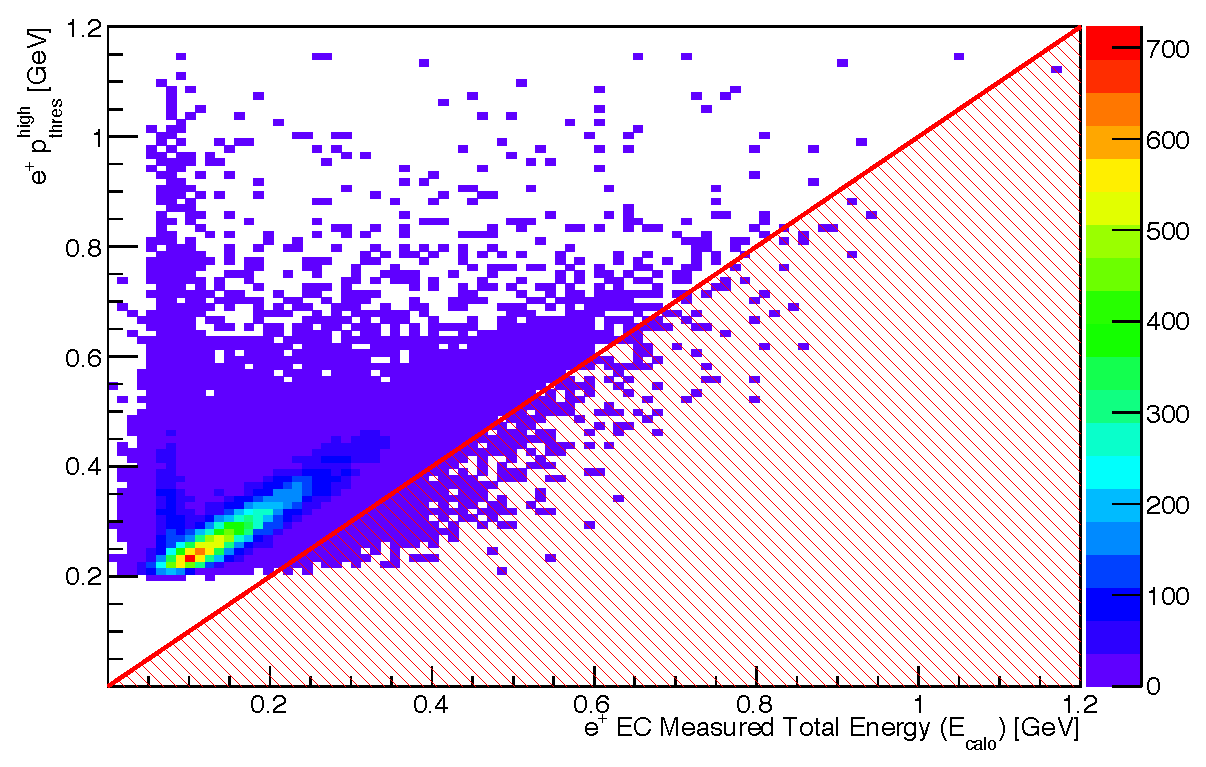
\includegraphics[width=0.45\columnwidth]{figures/lepton/Pip_EChighcut.eps}
\caption[\abbr{EC} Deposited Energy Comparison to Track Momentum for e$^+$ from π$^0$ Events]{\label{fig:islep.pipECcut}Plot of energy deposited measured by \abbr{EC} vs. track momentum p$\mathrm{_{thres}^{high}}$ for positrons from π$^0$ events without the \desg{g7} lepton \abbr{EC} \abbr{PID} scheme applied. The red region depicts the cut that would reject events in the \desg{g7} lepton \abbr{EC} \abbr{PID} scheme. Image source:~\cite{clas.thesis.kunkel}}
\end{center}\end{figure}



\FloatBarrier
